Now that the concepts have been presented, let us have a look at how these can be used to create a program. We will take the code from Hello World, and use a compiler to turn this code into a program that we can then execute. This process is the same for large and small programs.

\subsection{Installing the Tools}
\label{subs:install}
Before we get started you will need to install a few tools on your computer. The good news is that all of the tools we need are free (and many are open source - meaning you could one day look at the code used to create these and contribute back to helping continue to make these tools awesome).

The tools we will include all of the tools we have covered in this chapter:

\begin{itemize}
   \item A \textbf{terminal} and \textbf{shell} used to run scripts, and 
   \item A \textbf{compiler} used to convert code into an executable program you can run,
   \item Visual Studio Code: A \textbf{text editor} designed to work with code,
   \item \textbf{SplashKit} - a set of tools and libraries that we can use to make more interesting programs as you start to learn to program. 
\end{itemize}

Installation instructions for Linux, macOS, and Windows can be found at \url{https://www.splashkit.io/articles/installation/}. Follow the instructions for your operating system, and at the language step you can choose to install either the C++ or Pascal compiler. Make sure to check that each step succeeds, and if you get stuck you can ask questions on the SplashKit forum (\url{https://splashkit.discourse.group}).

If you cannot get these working, then there is a Virtual Machine that is also available that comes with all of the software preinstalled. You can download this VM, and open and run it using something like VirtualBox (\url{https://www.virtualbox.org}) (which is free), VMware (\url{https://www.vmware.com}), or Parallels (\url{https://www.parallels.com/}).

\clearpage
\subsection{Creating a Project with the SplashKit Manager: skm} % (fold)
\label{sub:skm}

SplashKit is an open source set of tools and libraries that can help you make more interesting applications as you learn to program. Within SplashKit the SplashKit Manager (\textbf{skm}) is a command line tool designed to take your compiler call, and add the extra options needed to link it with the SplashKit library. So when you use \textbf{skm}, you add the text `skm' to the start of the instruction in the Terminal. Let's have a look at how this works.

The best way to get started with a SplashKit program is to create a new folder (directory) in your file system that will be used to store the code and other files related to that program. The SplashKit manager can be used to create an empty program file along with files that store setings for Visual Studio Code.

\csection{
The following commands create a \emph{MyProject} folder, setup a new C++ project, and then compile it into a program.

\bashcode{lst:c-create-project}{Creating a C++ project with skm.}{code/c/program-creation/create-cpp-project.sh}
}

\passection{
The following commands create a \emph{MyProject} folder, setup a new Pascal project, and then compile it into a program.

\bashcode{lst:pas-create-project}{Creating a Pascal project with skm.}{code/pascal/program-creation/create-fpc-project.sh}
}

Now that you have the project started, we can edit the code to make the program do something interesting.

\clearpage
\subsection{Making the Hello World Program} % (fold)
\label{sub:compiling_code}

\lref{lst:hello-world-c} and \lref{lst:hello-world-pas} show the source code for the Hello World program. To make this into a program you need to:

\begin{enumerate}
  \item Write the code into the program code file.
  \item Save the file.
  \item Compile it.
\end{enumerate}

Step 1 and 2 can be accomplished with any text editor, but the best ones to use highlight your code. Each programming language has rules that determine how its code must be structured, known as the language's \textbf{syntax}. Programming editors, such as Visual Studio Code, make use of this structure to help visually format the code to make it easier to read. This is called \textbf{syntax highlighting}. This highlighting can help you identify any little mistakes you make. 

\fref{fig:cpp-example} shows the Hello World code in Visual Studio Code with C++, which has a consistent look across all platforms. The figure also includes the command line instructions needed to setup a new SplashKit C++ project, and compile it.

\begin{figure}[htbp]
   \centering
   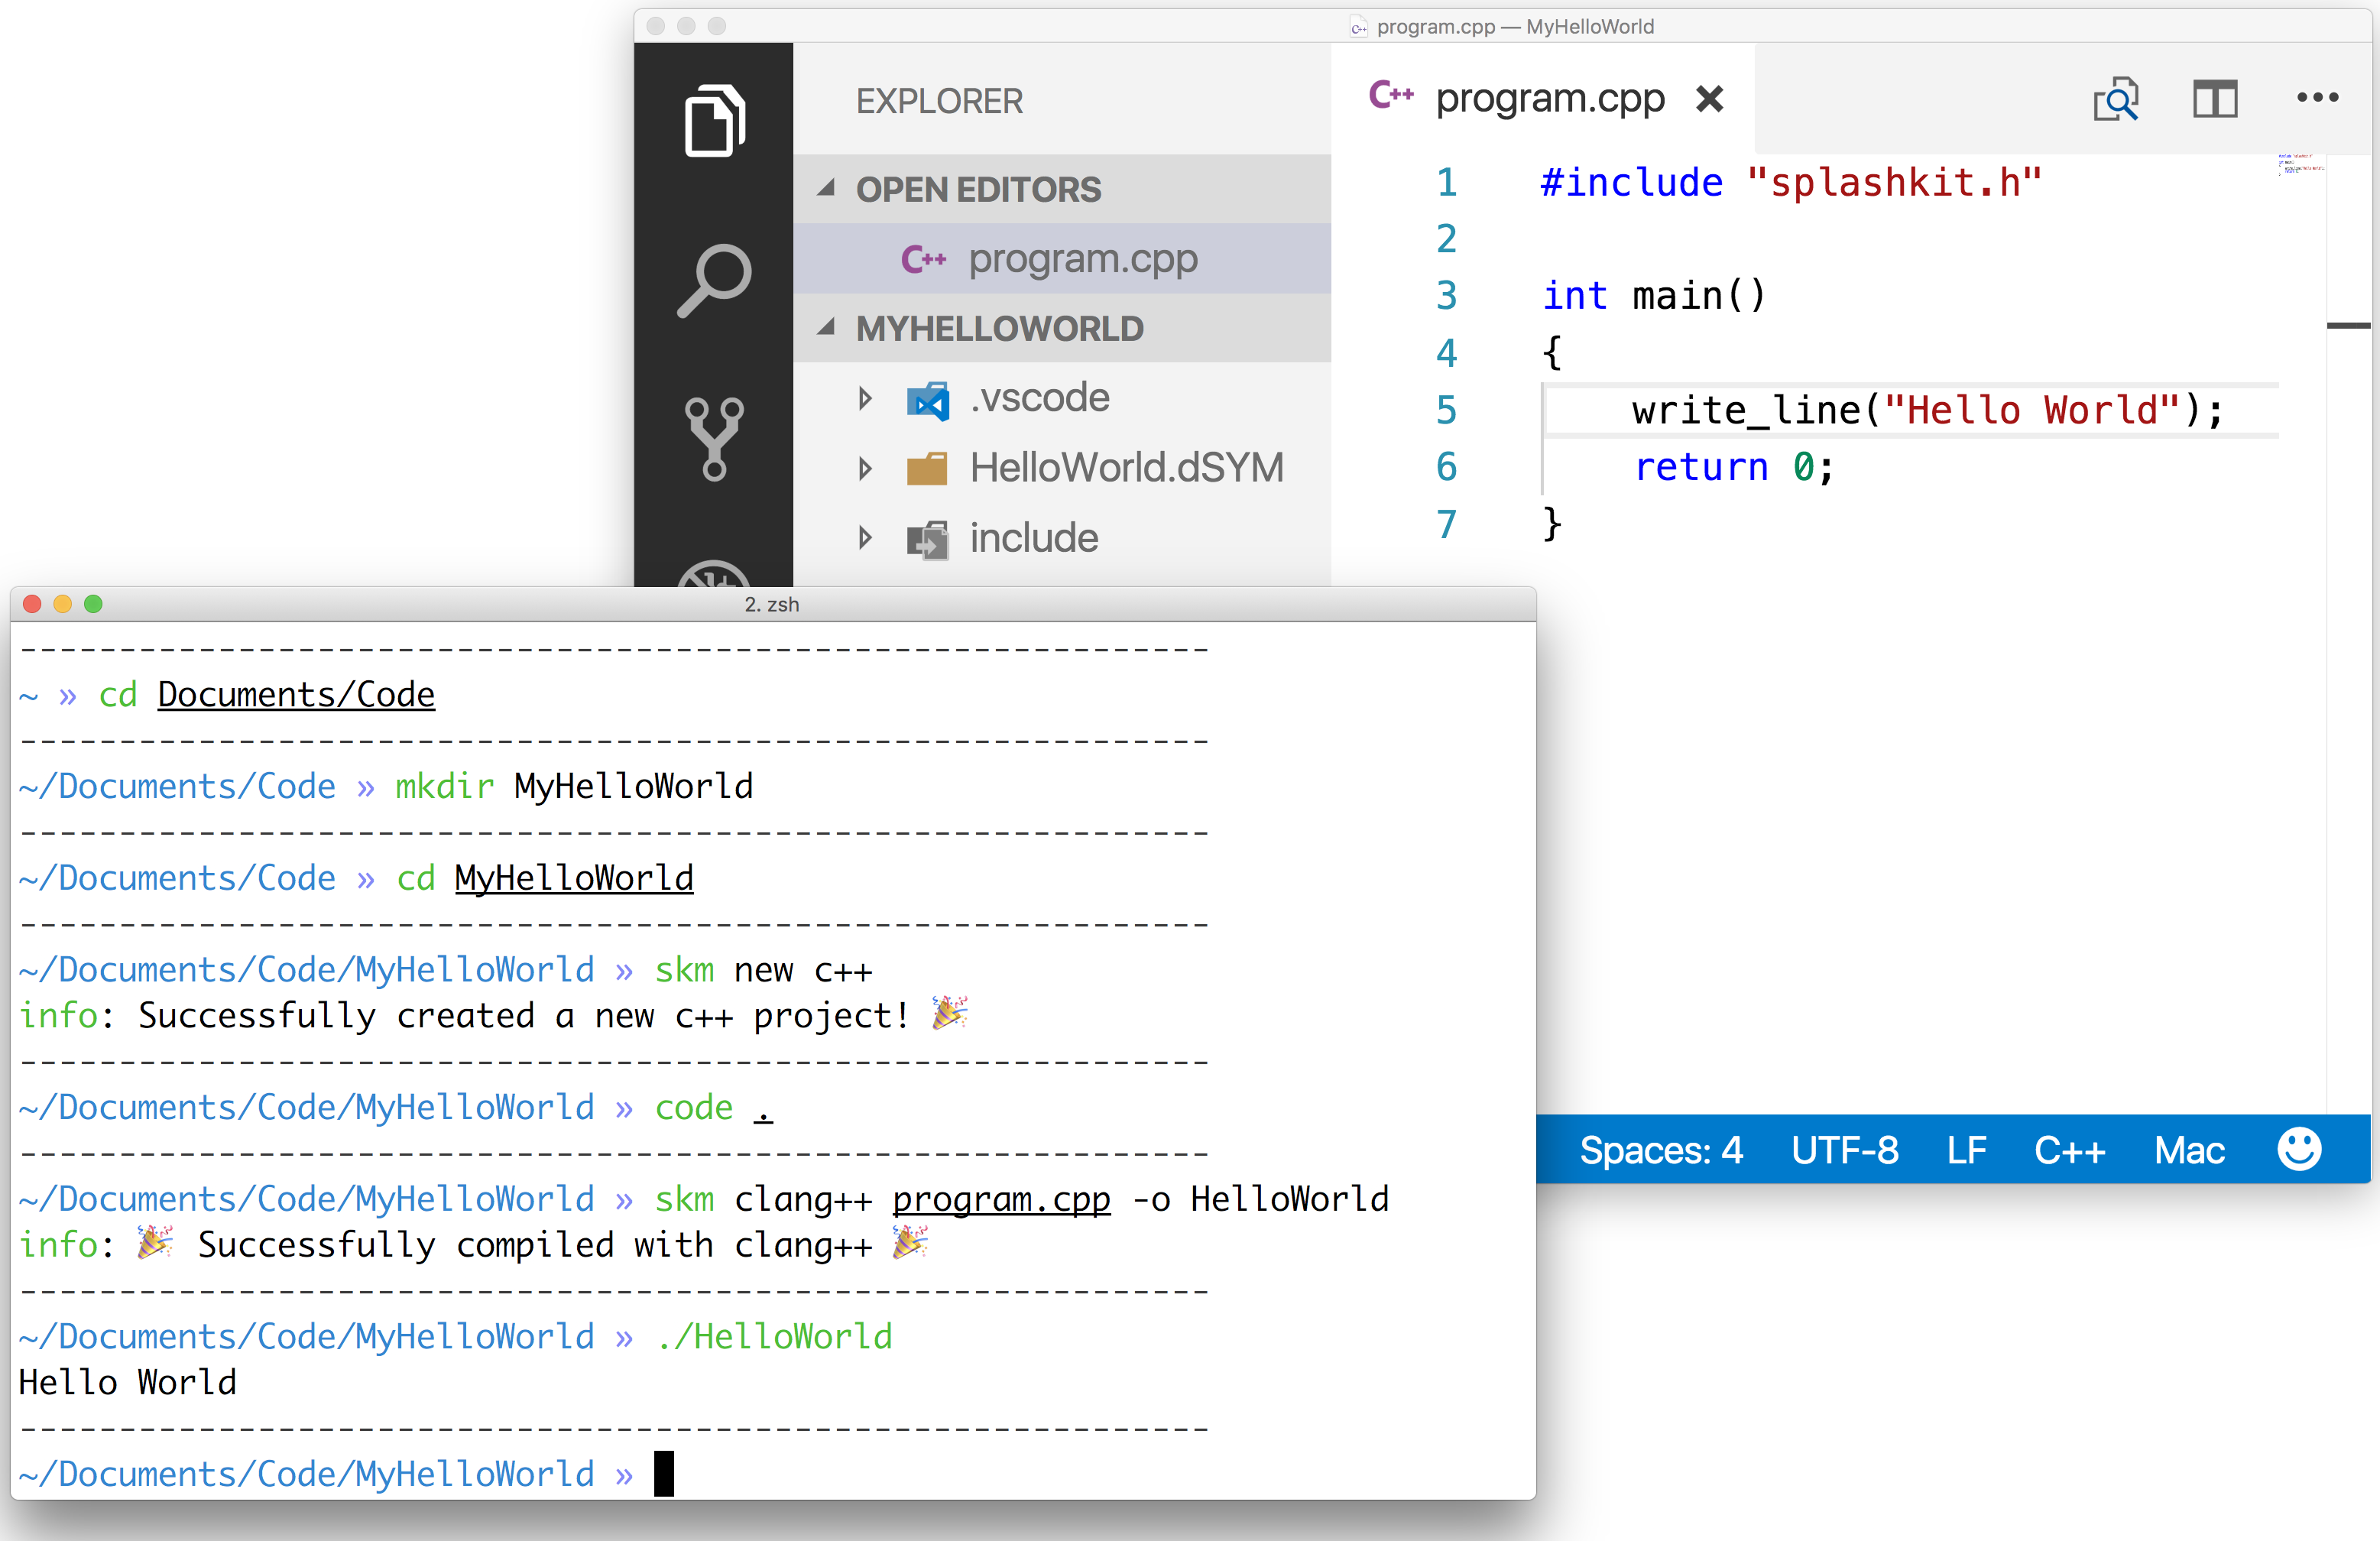
\includegraphics[width=0.8\textwidth]{./topics/programs-and-compilers/images/CppExample} 
   \caption{Editing and Compiling C++ code in Visual Studio Code}
   \label{fig:cpp-example}
\end{figure}

\fref{fig:fpc-example} shows the Hello World code in Visual Studio Code, which has a consistent look across all platforms. The figure also includes the command line instructions needed to setup a new SplashKit Pascal project, and compile it.

\begin{figure}[htbp]
   \centering
   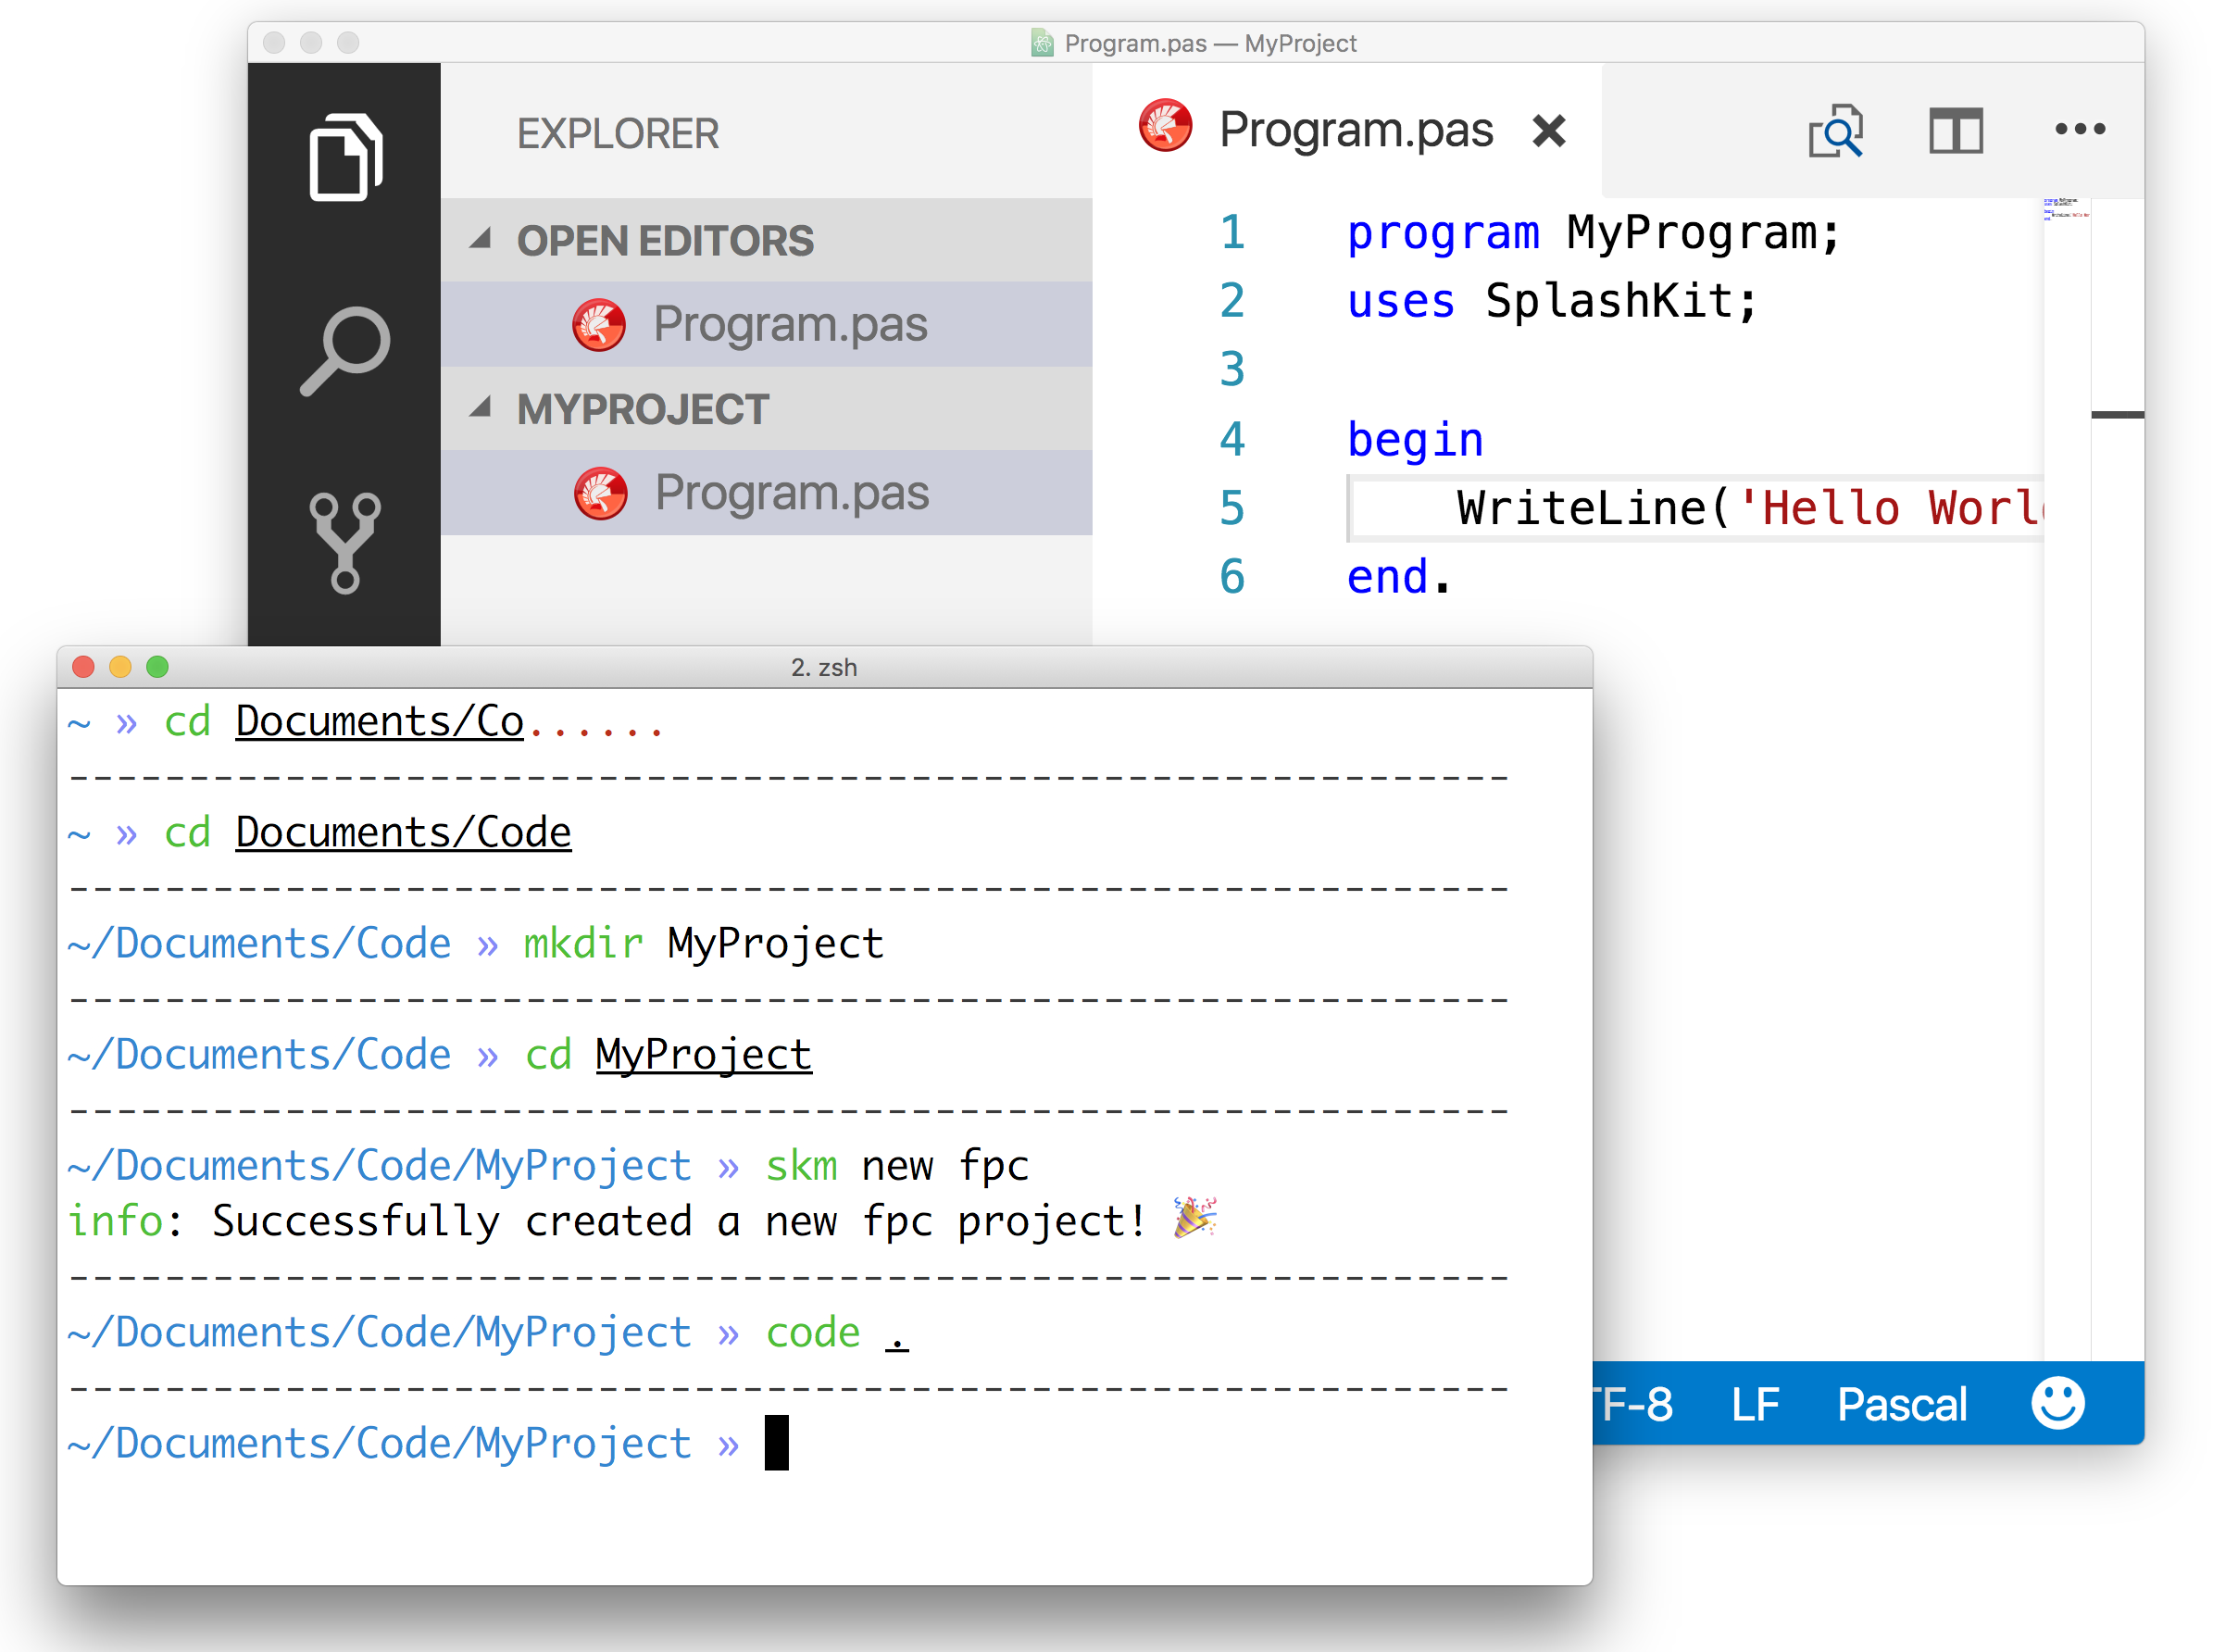
\includegraphics[width=0.8\textwidth]{./topics/programs-and-compilers/images/FpcExample} 
   \caption{Editing and Compiling Pascal code in Visual Studio Code}
   \label{fig:fpc-example}
\end{figure}

Use Visual Studio Code to open the \textbf{folder} that contains your project. This will give you access to that project's files and configure Visual Studio Code using the settings that skm has provided.

\clearpage
\subsubsection{Compiling the Code} % (fold)
\label{ssub:running_the_compiler}

Once you have saved the code it is time to compile your program. For this you are going to need switch back to the \nameref{sub:terminal} (or open a new one if you have closed it - reemmber to change into the directory where you saved the source code file). 

When you run the compiler you need to give it two kinds of information: options, and the names of the files to compile. The compiler will read the code in the files you give it, and convert this to machine code as shown in \sref{sub:source_code_and_the_compiler} \nameref{sub:source_code_and_the_compiler}. The exact command you use depends on the language and compiler you are running.

\csection{
The C++ compiler we will be using is called \textbf{clang++} (or \textbf{g++} the \textbf{GNU C++ Compiler}). The command you need to run in the Terminal is shown in Listing \ref{lst:compile-hello-world-c}. The \emph{-o name} option tells the compiler the name of the program file to create. In our example this will compile the code in \emph{hello-world.cpp} and save the machine code into a program called \emph{HelloWorld}.

\bashcode{lst:compile-hello-world-c}{Compiling C code.}{code/c/program-creation/compile-hello-world.sh}
}

\passection{
The Pascal compiler we will be using is called \textbf{fpc}, which stands for the \textbf{Free Pascal Compiler}. The command you need to run in the Terminal is shown in Listing \ref{lst:compile-hello-world-pas}. The \emph{-S2} option is used to tell fpc to compile using the latest `Free Pascal' version of the language. In our example this will compile the code in \emph{HelloWorld.pas} and save the machine code into a program called \emph{HelloWorld}, which it gets from the name of the Pascal file.

\bashcode{lst:compile-hello-world-pas}{Compiling Pascal code.}{code/pascal/program-creation/compile-hello-world.sh}
}

Once the code compiles, you will have a program you can run! Running the program will load it into memory, and start it running through the steps you coded. In this case, the HelloWorld program will output the text `\texttt{Hello World!}' to the Terminal. To run the program you need to use its file name. The command you need to enter is shown in \lref{lst:run-hello-world}, and in \fref{fig:run-helloworld}. The \texttt{./} before the file tells Bash to look in the current directory for the program.

\bashcode{lst:run-hello-world}{Bash command to run HelloWorld}{topics/programs-and-compilers/run-hello-world.sh}

\begin{figure}[h]
   \centering
   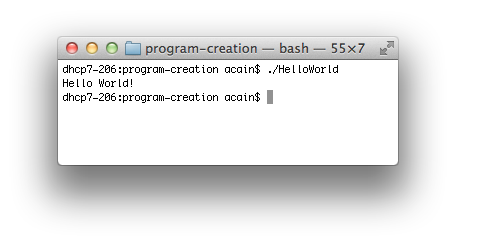
\includegraphics[width=0.7\textwidth]{./topics/programs-and-compilers/images/HelloWorld} 
   \caption[Hello World Terminal]{Hello World run from the Terminal}
   \label{fig:run-helloworld}
\end{figure}

% subsubsection running_the_compiler (end)

\subsubsection{When things do not work} % (fold)
\label{ssub:when_things_do_not_work}

Compilers are very specific about the code you give it. If the source code you try to compile does not follow all of the syntax rules of the language then the compiler will fail, and end with an error message. These errors, called \textbf{syntax errors}, could be as small as missing a semicolon (;), or misspelling a name. To get your program to compile you will need to correct any syntax errors the compiler finds in your code.

\begin{figure}[h]
   \centering
   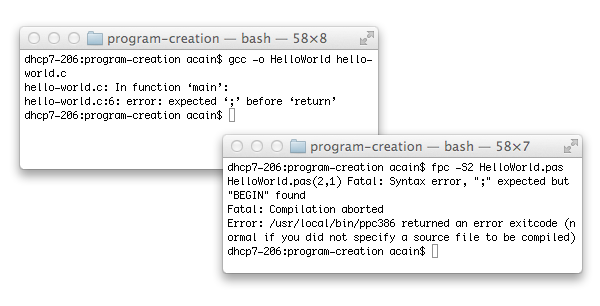
\includegraphics[width=0.8\textwidth]{./topics/programs-and-compilers/images/SyntaxErrors} 
   \caption{These Terminals show some syntax errors from programs that are missing a single semicolon (;)}
   \label{fig:syntax-errors}
\end{figure}

\fref{fig:syntax-errors} shows an example output caused by removing a single semicolon from the Hello World program's code. The numbers in the error messages give you an idea of where the compiler got to when it encountered the error. So the text \texttt{hello-world.c:6:} output from the C compiler indicates that the compiler got to line 6 before it encountered the error. The text \texttt{HelloWorld.pas(2,1)} output from the Pascal compiler indicates that it got up to line 2 character 1 before it encountered the error.

When the compiler encounters these issues it does not create the executable program. You need to learn to use these error messages to help you locate errors in your code, so that you can fix them, and then run the compiler again to generate your program.

\mynote{
\begin{itemize}
  \item Syntax errors are very common. Do not worry when this occurs to you.
  \item Always start with the first error. The compiler will try to continue compiling your code after it finds an error. This can mean that later errors do not really exist, once you fix the earlier ones.
  \item Unfortunately compiler error messages are not always very clear on what the cause of the error is. You need to learn how to read and understand these messages.
  \item To get good at programming requires lots of practice.
\end{itemize}
}

Here are a couple of things to check if you have compiler errors with the Hello World program:

\begin{itemize}
   \item Spaces in filename - avoid spaces in file names. The terminal uses spaces to separate different values in its instructions. In this context a space will then separate two values, rather than being captured as a space within the filename. If you do want a space use hyphens, or change case. For example \texttt{hello-world.cpp} or \texttt{HelloWorld.cpp} - there is no space here, but you can see the different words clearly.
   \item Missing semicolons - this is easy to do. Check for a missing \texttt{;} at the end of the previous line.
   \item Identifier not found - check the name you are using in the code. Most likely it is a small error. Compilers are often case sensitive, so WriteLine and writeline are different names.
   \item If you get errors with the hello world code, double check against the code provided.
\end{itemize}


% subsubsection when_things_do_not_work (end)



% section the_compiler (end)
